\documentclass[12pt,letterpaper]{article}

\usepackage[utf8]{inputenc}
\usepackage[T1]{fontenc}
\usepackage[spanish,es-noindentfirst]{babel}
\usepackage[margin=2.5cm]{geometry}
\usepackage{graphicx}
\usepackage{booktabs}
\usepackage{array}
\usepackage{xcolor}
\usepackage{enumitem}
\usepackage{float}
\usepackage{caption}
\usepackage{hyperref}

\definecolor{tecnico}{HTML}{1C6B63}
\definecolor{grisnota}{HTML}{5B6572}

\hypersetup{
    colorlinks=true,
    linkcolor=black,
    citecolor=black,
    urlcolor=tecnico,
    pdftitle={Propuesta - Conjunto de datos anotado de tejidos en ulceras de pie diabetico},
    pdfauthor={Adrian Emiliano Beltran Fernandez}
}

\captionsetup{font=small,labelfont=bf}
\setlist{itemsep=2pt,topsep=3pt}
\addto\captionsspanish{\renewcommand{\tablename}{Tabla}}

% Recuadro para notas dirigidas al lector tecnico, para que el lector clinico
% pueda saltarselas sin perder el hilo.
\newcommand{\notatecnica}[1]{%
    \par\vspace{4pt}
    \noindent\colorbox{tecnico!8}{%
        \parbox{\dimexpr\linewidth-2\fboxsep}{%
            \small\textcolor{tecnico}{\textbf{Nota técnica.}} \small #1}}%
    \par\vspace{4pt}
}

\title{\textbf{Propuesta de trabajo:\\
Construcción de un conjunto de datos anotado de tejidos\\
en úlceras de pie diabético}\\[0.4em]
\large Documento para discusión con el equipo clínico y el tutor}

\author{Adrián Emiliano Beltrán Fernández\\
\small Estudiante de Física Biomédica, Facultad de Ciencias, UNAM\\[0.6em]
\small Tutor: Dr.\ José Eduardo Chairez Veloz (Facultad de Ciencias, UNAM)\\
\small Asesoría clínica: Dr.\ Gerardo \textit{[apellido]} y Facultad de Enfermería y Obstetricia, UNAM\\
\small Proyecto derivado de PAPIIT IN115825}

\date{Ciudad de México, \today\\[0.3em]
\small\textit{Versión de propuesta --- sujeta a revisión con el equipo médico}}

\begin{document}

\maketitle

\begin{abstract}
\noindent Este documento propone construir un conjunto de datos (\textit{dataset}) de fotografías
clínicas de úlceras de pie diabético (UPD) en el que un equipo de especialistas marque, sobre cada
imagen, la localización exacta de cada tipo de tejido. Se explica \textbf{qué se pide anotar}
(cinco tipos de tejido y una distinción binaria tejido/no--tejido), \textbf{cómo se hace}
(trazado de contornos asistido por computadora en MATLAB), \textbf{por qué conviene hacerlo de esta
forma} y \textbf{qué valor científico tendría el resultado}: sería apenas el tercer conjunto de datos
de este tipo disponible públicamente en el mundo y el primero originado en América Latina. El documento
está escrito para ser entendible tanto por personal clínico como por personas con perfil técnico;
las secciones más técnicas están señaladas y pueden omitirse sin perder el hilo.
\end{abstract}

\tableofcontents

\vspace{1em}

% =====================================================================
\section{Resumen ejecutivo}
% =====================================================================

\begin{itemize}
  \item \textbf{Qué se busca.} Un modelo computacional que, a partir de una fotografía de una úlcera,
        indique \emph{qué tejidos hay y dónde están} (granulación, fibrina, tejido necrótico, callo,
        y el estado de la piel de alrededor). Esto apoya decisiones clínicas como cuándo desbridar,
        cómo elegir el apósito y cómo seguir la evolución de la herida.
  \item \textbf{Qué falta hoy.} El proyecto tiene ya toda la parte computacional montada (modelos,
        entrenamiento, evaluación), pero las anotaciones que se hicieron hasta ahora fueron
        \emph{aproximadas} (una caja alrededor de la zona) y con criterios que cambiaron a mitad del
        proceso. Eso limita lo que el modelo puede aprender y, sobre todo, impide \emph{medir} con
        rigor qué tan bien localiza cada tejido.
  \item \textbf{La propuesta.} Rehacer las anotaciones de forma \textbf{precisa}: trazar el contorno
        real de cada tejido en cada imagen. Se hace una sola vez y de ahí se derivan automáticamente
        todas las versiones más simples que los experimentos necesiten.
  \item \textbf{Qué se pide al equipo médico.} Trazar, sobre cada foto, el contorno de cinco tipos de
        tejido, con una herramienta que asiste el trazado (se explica en el Anexo~\ref{anexo:matlab}).
        Y aportar el criterio clínico para definir bien cada tejido.
  \item \textbf{Qué se obtendría.} Un conjunto de datos mexicano, con diversidad de tonos de piel
        (algo que los datasets existentes casi no tienen), que llenaría vacíos concretos señalados
        por las revisiones recientes del área y serviría de base para la tesis y para al menos una
        publicación.
\end{itemize}

% =====================================================================
\section{Contexto: qué se está construyendo y por qué}
% =====================================================================

Las úlceras de pie diabético son una de las principales causas de amputación de miembro inferior. Su
evaluación en la práctica todavía depende de la inspección visual y de la experiencia de quien
observa, lo que introduce variabilidad entre observadores y retrasa la detección de deterioro.

Este proyecto desarrolla un sistema de análisis de imagen que apunta a dos salidas:

\begin{enumerate}
  \item \textbf{Clasificación}: decir qué tejidos están presentes en la foto.
  \item \textbf{Localización}: decir \emph{dónde} está cada tejido, con una precisión útil para el
        clínico (idealmente parecida a una segmentación, es decir, píxel por píxel).
\end{enumerate}

La primera salida ya funciona razonablemente. La segunda no: con las anotaciones actuales, el modelo
acierta \emph{qué} tejidos hay pero no aprende \emph{dónde} están. La razón, comprobada en los
experimentos, es que las anotaciones por caja no le dan al modelo la información espacial que
necesita, y además no existe una ``respuesta correcta'' contra la cual medir la localización. La
propuesta de este documento resuelve las dos cosas a la vez.

\notatecnica{El sistema base es un modelo de \textit{Multiple Instance Learning} con atención (Ilse
et al., ICML 2018) sobre un extractor \textit{MobileNetV2}. El diagnóstico del problema de
localización (mapas de atención casi uniformes; mediana de contraste $\approx 0.04$ en escala 0--1)
está documentado en la bitácora del proyecto, Parte III. La anotación densa habilita (i) una
referencia para medir localización con Dice/IoU, (ii) supervisión mixta tipo MS-CLAM, y (iii)
generar etiquetas débiles de forma consistente y automática.}

% =====================================================================
\section{Qué se le pide anotar al equipo médico}
% =====================================================================

\subsection{Anotación aproximada (lo anterior) frente a anotación precisa (lo que se propone)}

Hasta ahora, anotar una imagen significaba dibujar una \textbf{caja rectangular} alrededor de la
úlcera y escribir una lista de los tejidos presentes. Es rápido, pero la caja no distingue un tejido
de otro dentro de ella, e incluye mucha piel sana ``de relleno''.

Lo que se propone es \textbf{trazar el contorno real de cada tejido} --- lo que en computación se
llama un \emph{polígono}: una figura cerrada hecha de puntos unidos, como un ``une los puntos''
alrededor del borde del tejido. El interior de ese contorno queda marcado como ese tejido. La
Figura~\ref{fig:debilfuerte} compara las dos formas.

\begin{figure}[H]
\centering
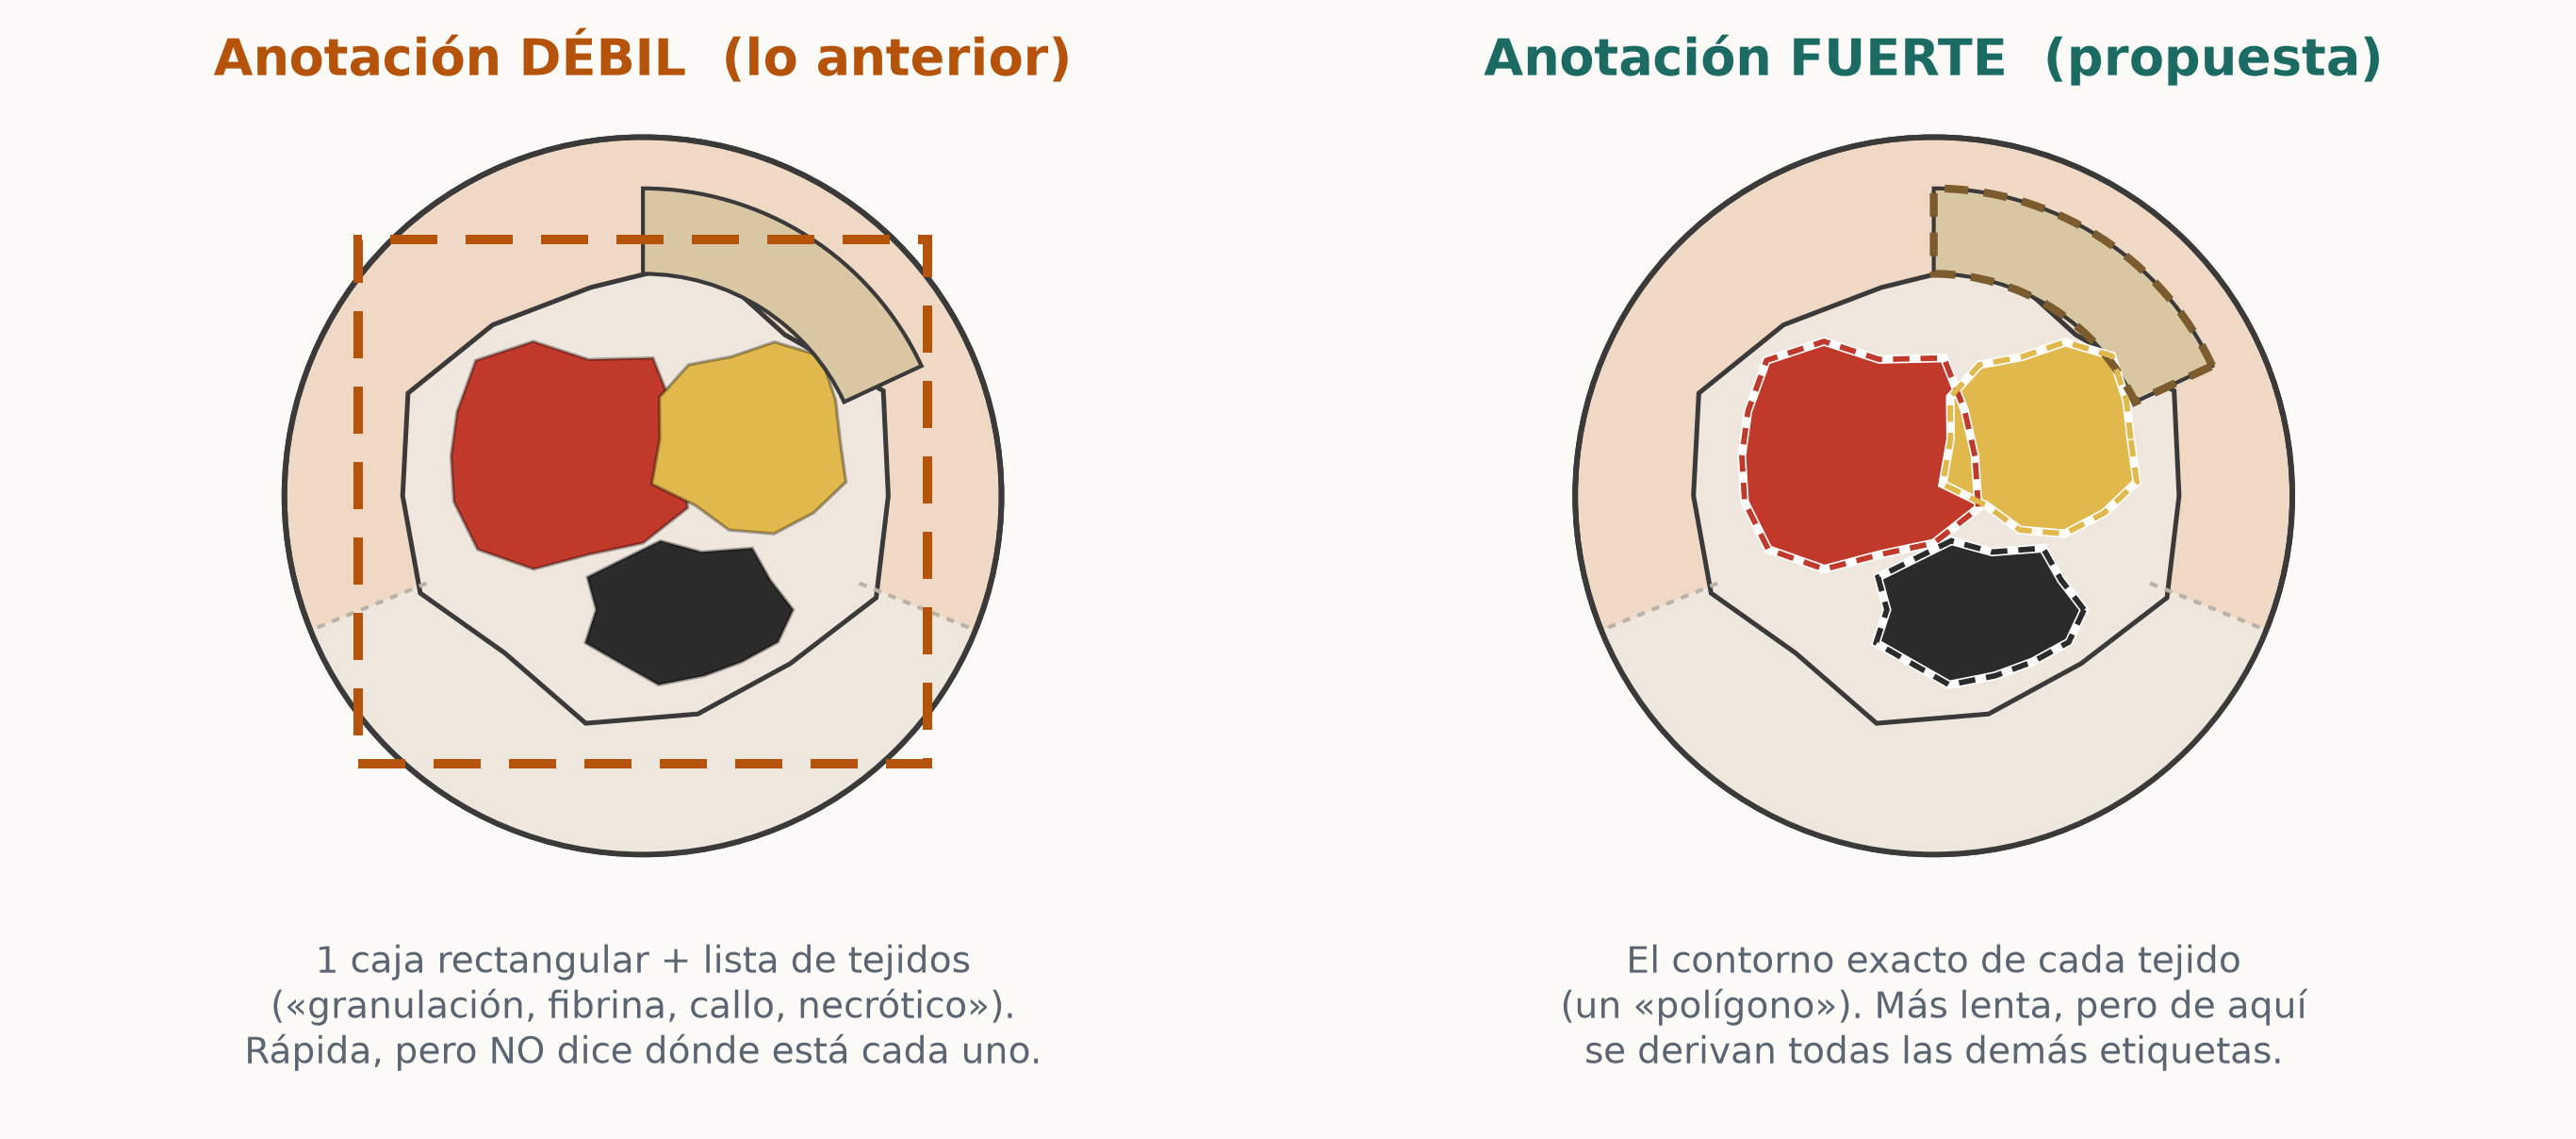
\includegraphics[width=\textwidth]{figuras/fig_debil_vs_fuerte.png}
\caption{Izquierda: anotación aproximada (una caja + lista de tejidos). Derecha: anotación precisa
(el contorno de cada tejido). Esquemas ilustrativos, no casos clínicos reales.}
\label{fig:debilfuerte}
\end{figure}

\subsection{Por qué precisa, y por qué una sola vez}

\begin{itemize}
  \item \textbf{Es consistente.} No depende del criterio del día ni de quién anotó: el contorno de un
        tejido es el contorno de ese tejido.
  \item \textbf{Permite medir.} Con el contorno real como referencia, se puede calcular con un número
        objetivo qué tan bien el modelo localiza cada tejido.
  \item \textbf{Se deriva hacia abajo, no hacia arriba.} De una anotación precisa se obtiene
        automáticamente la lista de tejidos por foto, la máscara binaria tejido/no--tejido, y
        cualquier otra versión simplificada. Al revés no se puede. Por eso se invierte el esfuerzo
        una sola vez, en la versión más completa.
\end{itemize}

% =====================================================================
\section{Los cinco tejidos propuestos}
% =====================================================================

Se propone anotar \textbf{cinco categorías}, elegidas por tres criterios simultáneos: (a) relevancia
clínica para evaluar la cicatrización; (b) evidencia en la literatura de que los modelos
\emph{sí} logran distinguirlas del resto; y (c) que aparezcan con frecuencia suficiente en un
conjunto de este tamaño. La Figura~\ref{fig:esquema} y la Tabla~\ref{tab:tejidos} las resumen.

\begin{figure}[H]
\centering
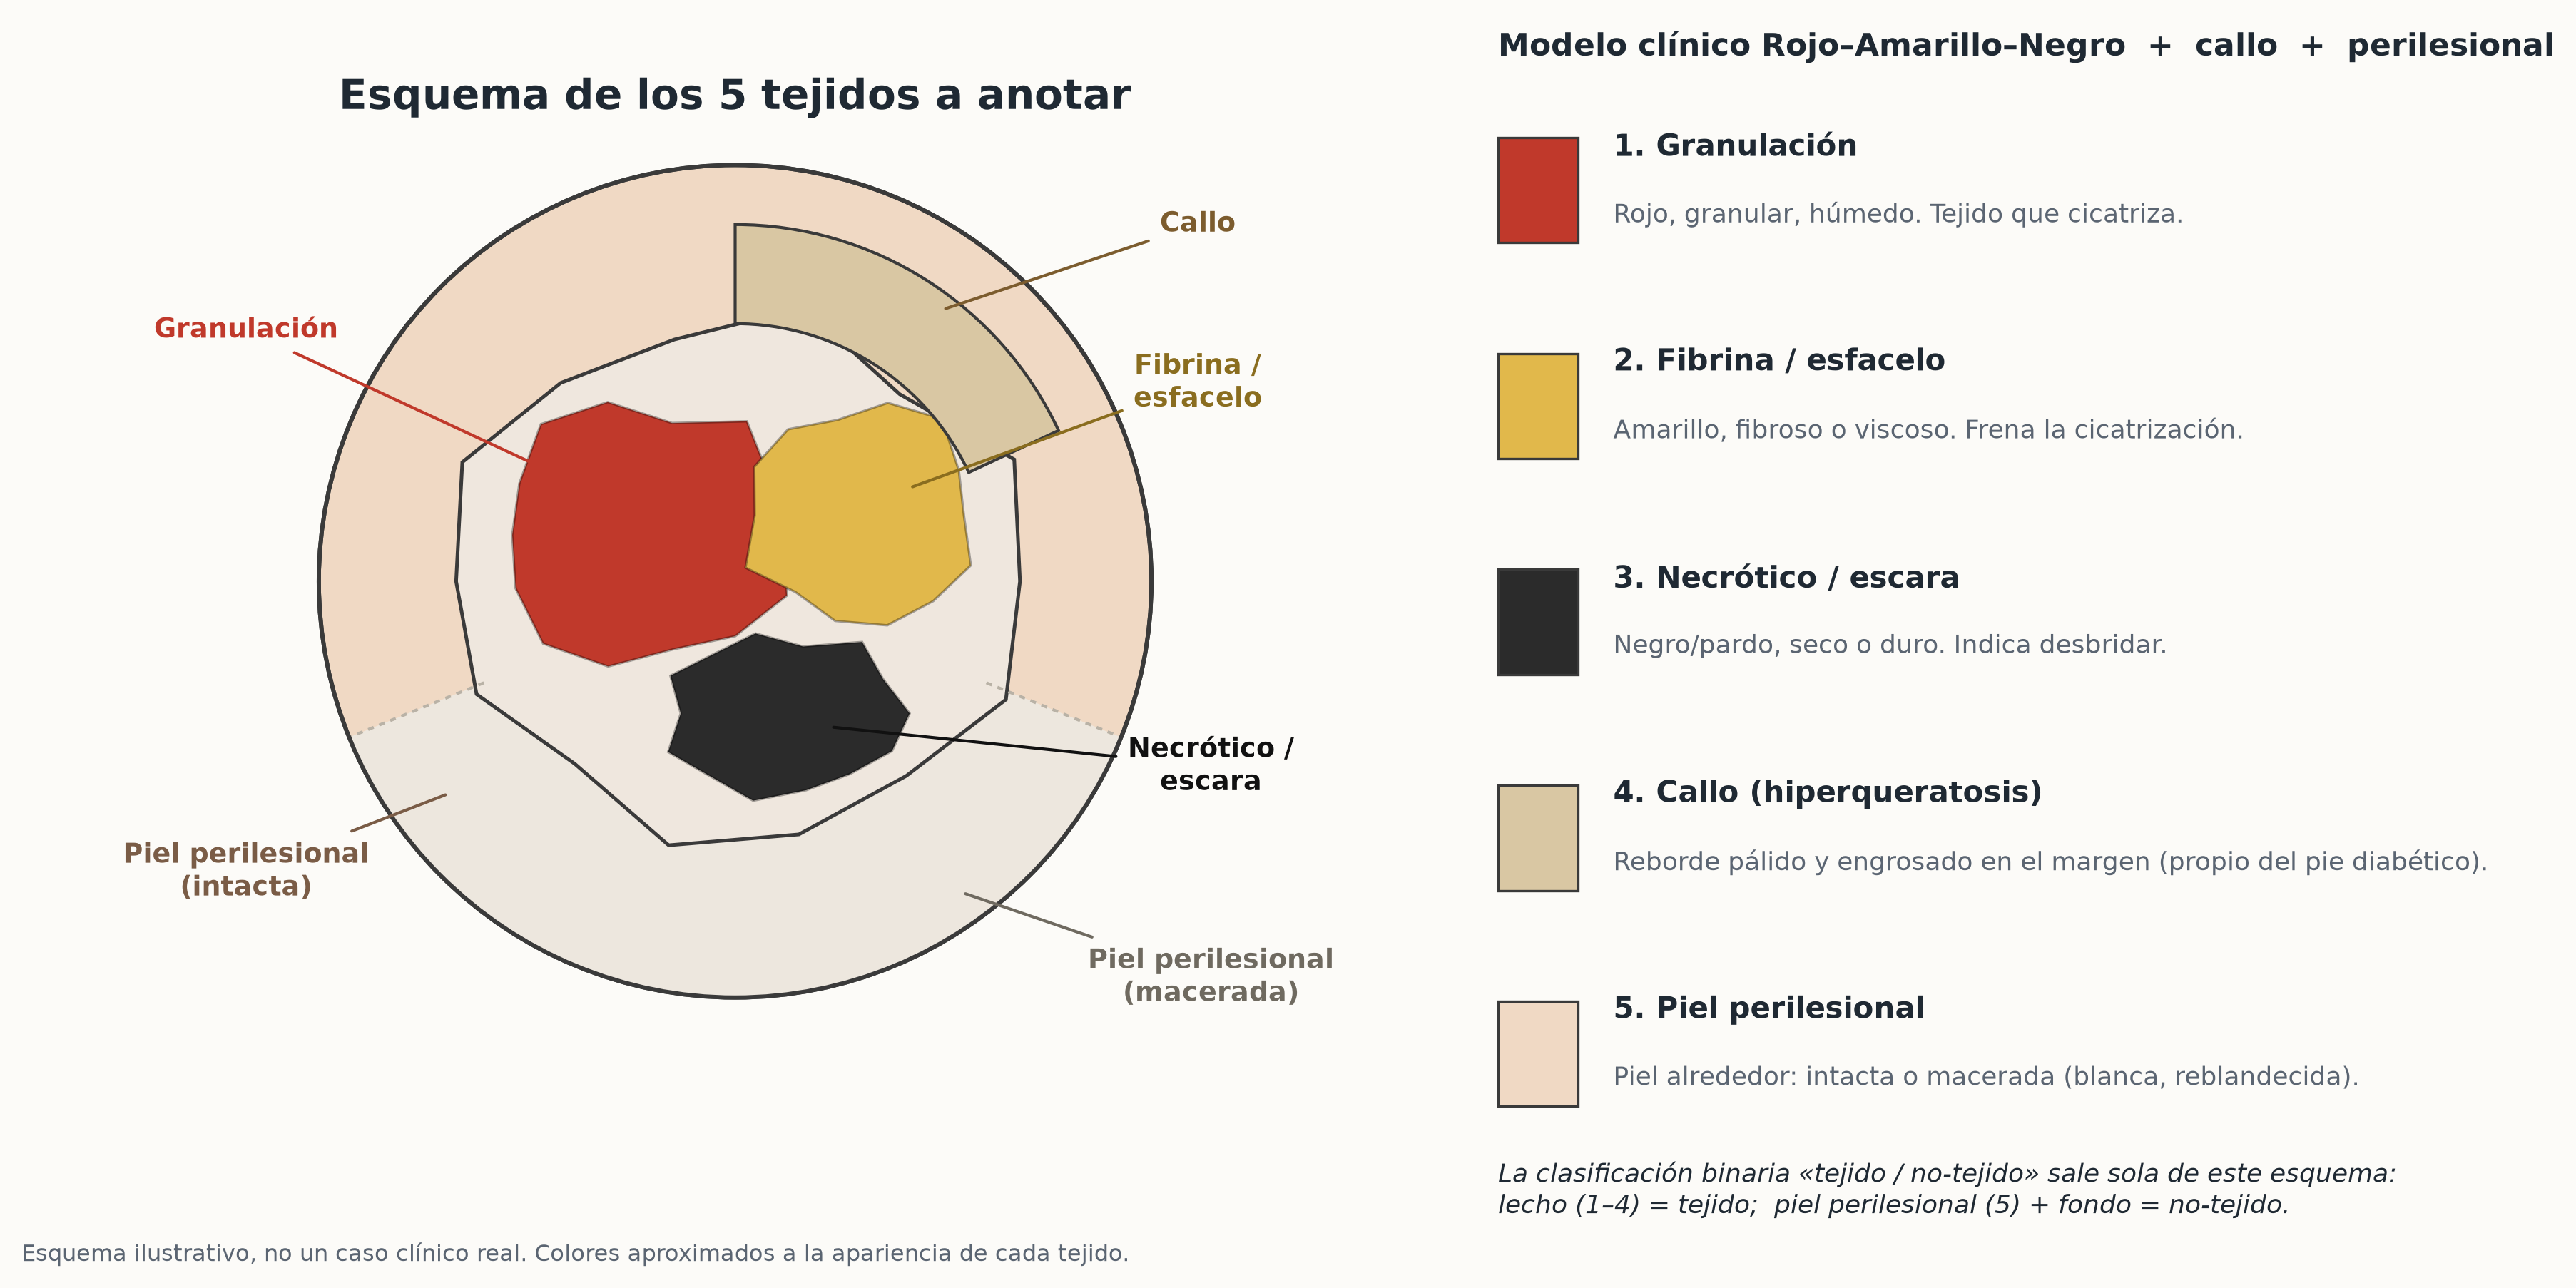
\includegraphics[width=\textwidth]{figuras/fig_esquema_5_tejidos.png}
\caption{Los cinco tejidos propuestos, sobre el modelo clínico clásico Rojo--Amarillo--Negro,
ampliado con el callo (propio del pie diabético) y con la piel perilesional. Esquema ilustrativo.}
\label{fig:esquema}
\end{figure}

\begin{table}[H]
\centering
\small
\caption{Las cinco categorías propuestas.}
\label{tab:tejidos}
\renewcommand{\arraystretch}{1.35}
\begin{tabular}{@{}p{2.6cm}p{4.6cm}p{6.6cm}@{}}
\toprule
\textbf{Categoría} & \textbf{Aspecto / definición clínica} & \textbf{Por qué se incluye} \\
\midrule
1. Granulación &
Rojo, granular, húmedo, brillante. Tejido sano que rellena la herida. &
Es el tejido que mejor distinguen todos los modelos publicados (Dice típico 0.70--0.91). Señal de
cicatrización. \\

2. Fibrina / esfacelo &
Amarillo o blanquecino, fibroso o viscoso, adherido al lecho. &
Marca estancamiento de la cicatrización y es criterio de limpieza/desbridamiento. Es el tejido más
difícil del lecho, pero medible (Dice 0.66--0.77 en trabajos recientes). \\

3. Tejido necrótico / escara &
Negro o pardo oscuro, seco y duro (escara) o húmedo. &
Indica necesidad de desbridamiento y riesgo de infección. Alto contraste visual $\Rightarrow$
los modelos lo distinguen bien cuando hay ejemplos suficientes. \\

4. Callo (hiperqueratosis) &
Reborde pálido, engrosado y seco en el margen de la herida. &
Propio del pie diabético; su presencia y grosor tienen valor pronóstico. Ya estaba en el trabajo
previo del grupo y en el dataset público DFUTissue. \\

5. Piel perilesional &
La piel inmediatamente alrededor de la úlcera: intacta, o \emph{macerada} (blanca, reblandecida por
humedad). &
Central para el manejo del borde y la elección del apósito. Está en \emph{todas} las fotos, lo que
equilibra el conjunto de datos, y define directamente la máscara binaria (ver abajo). \\
\bottomrule
\end{tabular}
\end{table}

\paragraph{Qué se deja fuera, y por qué.} El \textbf{hueso} y el \textbf{tendón} expuestos son
clínicamente muy importantes, pero aparecen tan poco en fotografías que ningún modelo logra
aprenderlos con un conjunto pequeño; se registran como observación libre pero no como categoría a
segmentar. La \textbf{hiperpigmentación} se descarta porque se confunde con el tono de piel del
paciente y puede introducir sesgo. \textbf{Epitelización}, \textbf{hipergranulación} y
\textbf{exudado} se dejan como posibles categorías futuras si el volumen de datos lo permite.

\paragraph{La clasificación binaria (tejido / no--tejido).} No es un trabajo aparte: sale sola del
esquema de cinco clases. El \emph{lecho} de la herida (categorías 1 a 4) es ``tejido''; la piel
perilesional (categoría 5) y el fondo de la foto son ``no--tejido''. Esta distinción binaria es la
que corresponde a la máscara de herida del trabajo previo del grupo, es la más robusta
estadísticamente con pocos datos, y sirve de resultado principal; la clasificación de los cinco
tejidos es el resultado más detallado y exploratorio.

% =====================================================================
\section{Cómo se anota, en la práctica}
% =====================================================================

La herramienta propuesta es \textbf{MATLAB} en su versión web (\textit{Image Labeler}), porque
funciona en cualquier computadora con un navegador --- incluidas las que no usan Windows --- y
porque el tutor y el estudiante ya cuentan con licencia. El paso a paso está en el
Anexo~\ref{anexo:matlab}.

El flujo completo, de la foto a los datos, se resume en la Figura~\ref{fig:flujo}:

\begin{figure}[H]
\centering
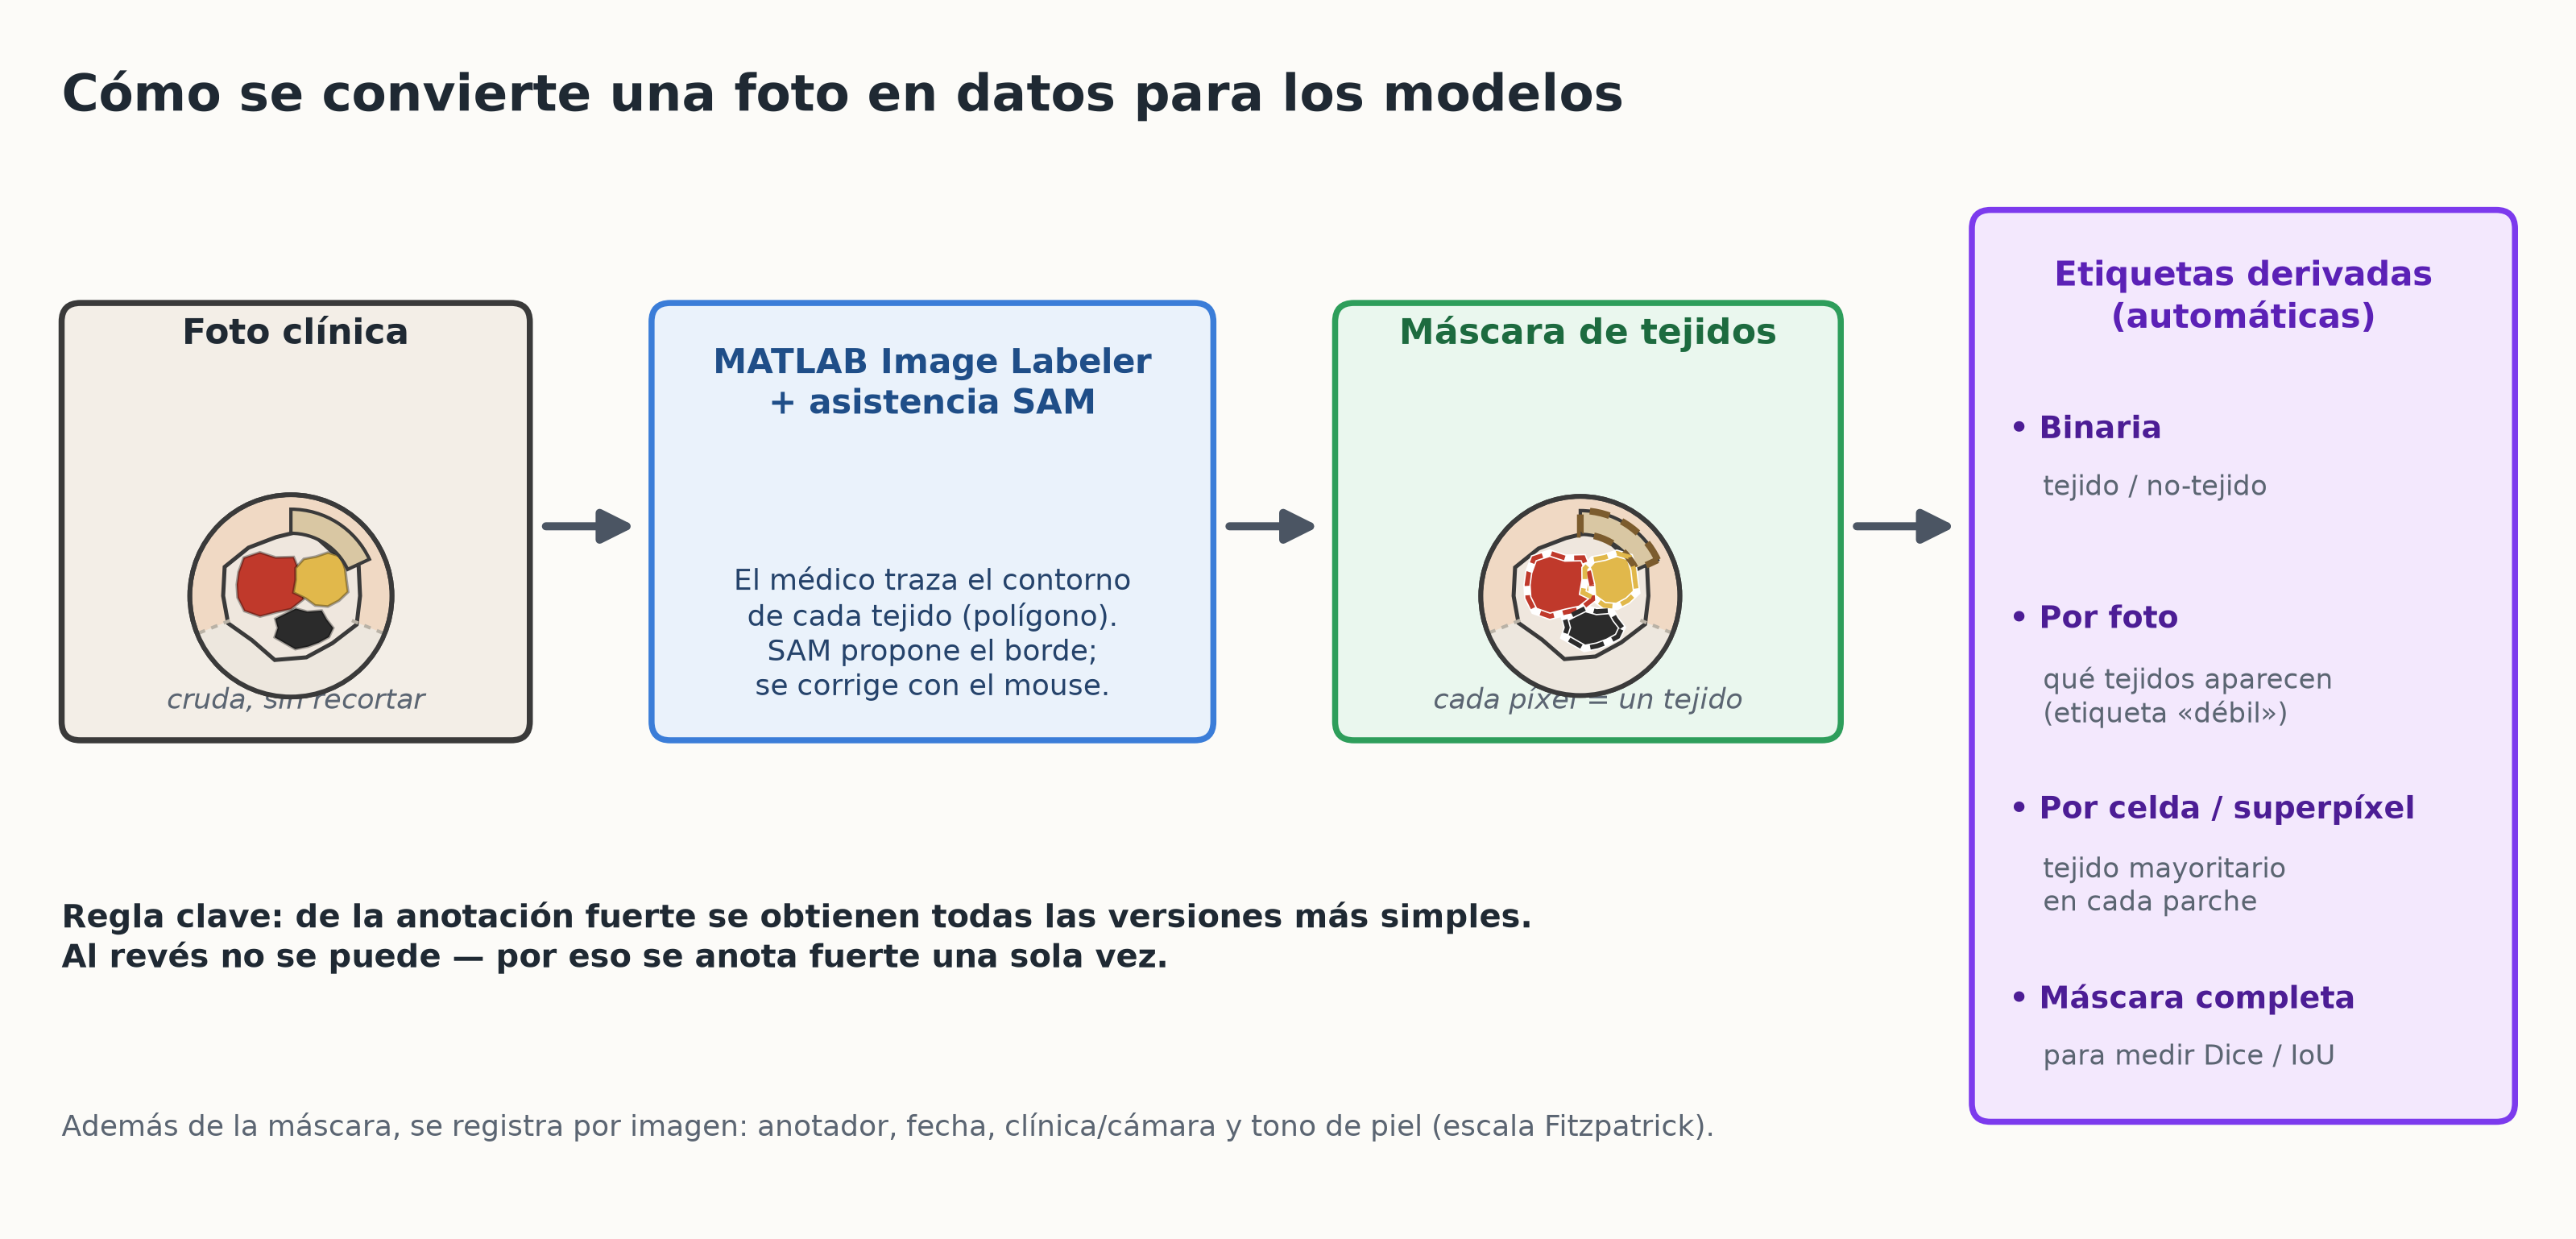
\includegraphics[width=\textwidth]{figuras/fig_flujo_anotacion.png}
\caption{De una fotografía clínica a los datos que usan los modelos. El equipo médico solo interviene
en el segundo paso (trazar los contornos). Todo lo demás es automático.}
\label{fig:flujo}
\end{figure}

\subsection{Criterios de anotación a acordar con el equipo clínico}

\begin{itemize}
  \item \textbf{Qué incluir y qué no.} Definir, con ejemplos, el límite entre fibrina y esfacelo
        (¿se unen en una sola categoría?), entre callo y piel perilesional engrosada, y entre
        maceración y piel sana húmeda.
  \item \textbf{Zonas dudosas.} Acordar qué hacer cuando un área tiene mezcla de tejidos o el borde
        no está claro: marcar el tejido predominante, o dejar sin marcar.
  \item \textbf{Piel perilesional.} Definir cuánta piel alrededor de la herida se incluye.
  \item \textbf{Consistencia entre anotadores.} Un subconjunto de imágenes (por ejemplo, 15--20)
        debe ser anotado \emph{de forma independiente por más de una persona}, para medir el grado de
        acuerdo entre especialistas. Esto no es burocracia: es un requisito de rigor que las
        revisiones del área señalan que casi nadie cumple, y refuerza mucho la validez del conjunto.
\end{itemize}

\subsection{Qué se registra además de la máscara}

Por cada imagen se anota: \textbf{quién} la anotó, \textbf{cuándo}, de \textbf{qué clínica o
cámara} proviene, y el \textbf{tono de piel del paciente} (escala de Fitzpatrick, si el clínico la
puede estimar). Esta información es necesaria para:

\begin{enumerate}
  \item auditar que el modelo funcione igual de bien en todos los tonos de piel;
  \item el componente de \emph{aprendizaje continuo} de la tesis, que estudia qué pasa cuando los
        datos llegan por lotes a lo largo del tiempo (de distintos anotadores o clínicas);
  \item la trazabilidad que exige cualquier publicación con datos clínicos.
\end{enumerate}

% =====================================================================
\section{Qué se lograría: el conjunto de datos como aporte científico}
% =====================================================================

\subsection{Qué conjuntos de datos existen hoy}

La Tabla~\ref{tab:datasets} resume los conjuntos de datos publicados de segmentación de heridas. La
lección es contundente: \textbf{solo existen dos conjuntos de datos de \emph{tejidos} de herida
disponibles públicamente en todo el mundo} (DFUTissue y WoundTissueSeg), ambos pequeños, ninguno
con licencia plenamente abierta (uno sin licencia, otro no comercial), ninguno de América Latina, y
casi ninguno con diversidad de tonos de piel. Un conjunto propio, publicado con una licencia
verdaderamente abierta, sería el más permisivo del área.

\begin{table}[H]
\centering
\footnotesize
\caption{Conjuntos de datos publicados de segmentación de heridas (selección). ``Binaria'' = solo
distingue herida de piel, sin tipos de tejido.}
\label{tab:datasets}
\renewcommand{\arraystretch}{1.3}
\begin{tabular}{@{}p{3.1cm}p{1.7cm}p{3.0cm}p{2.2cm}p{3.0cm}@{}}
\toprule
\textbf{Conjunto} & \textbf{Imágenes} & \textbf{Tejidos anotados} & \textbf{Licencia} & \textbf{Origen} \\
\midrule
DFUTissue (2024) & 110 (+600 sin etiqueta) & 3: granulación, callo, fibrina & Sin licencia (uso $\to$ citar el artículo) & EE.UU.\ (Milwaukee) \\
WoundTissueSeg (2025) & 147 (13 públicas; resto a petición) & 6: granulación, esfacelo, maceración, necrosis, hueso, tendón & CC BY-NC-SA 4.0 (no comercial) & Mixto \\
Huttunen et al.\ (2026) & 362 & 4--5 & A petición & Finlandia (solo piel clara) \\
Morgado et al.\ (2025) & --- & 3: granulación, esfacelo, escara & --- & Portugal \\
WING--MTL (2026) & 350 & 4: granulación, esfacelo, epitelio, necrosis & Restringida & Corea del Sur \\
Zhao et al.\ (2025) & 671 & $\sim$6 & Privada & Asia \\
\midrule
FUSeg (2021) & 1\,210 & Binaria & Pública & EE.UU. \\
DFUC 2022 & 4\,000 & Binaria & Acuerdo de uso & Reino Unido \\
\midrule
\textbf{Propuesto (este proyecto)} & \textbf{60--270} & \textbf{5 + binaria} & \textbf{Abierta (planeada)} & \textbf{México, piel diversa} \\
\bottomrule
\end{tabular}
\end{table}

\subsection{Por qué el nuestro sería relevante para el estado del arte}

\begin{itemize}
  \item \textbf{Sería apenas el tercer conjunto de datos de tejidos de UPD disponible públicamente en
        el mundo, y el primero de América Latina} --- y, publicado con licencia abierta, el más
        reutilizable de los tres. Aunque tenga ``solo'' 60--270 imágenes, eso ya lo pone a la par de
        DFUTissue (110) y WoundTissueSeg (147), que son las referencias del campo.
  \item \textbf{Diversidad de tonos de piel.} Las revisiones recientes (Yu et al., 2026;
        Reifs Jiménez et al., 2025) señalan explícitamente que los datasets existentes son
        homogéneos en tono de piel y que esto introduce sesgo. Una cohorte mexicana aporta justo esa
        diversidad.
  \item \textbf{Permite comparaciones que nadie ha hecho.} Con las tres categorías compartidas
        (granulación, callo, fibrina) se puede entrenar en México y validar en DFUTissue, y
        viceversa: es el primer estudio de generalización entre poblaciones para tejidos de herida.
  \item \textbf{Rigor de anotación.} Con anotación por varios especialistas y medida de acuerdo
        entre ellos, cubre otro vacío que las revisiones nombran (la mayoría de los trabajos no
        documenta cómo se generó la ``respuesta correcta'').
\end{itemize}

\subsection{Qué se podría lograr con el modelo}

Como referencia realista: el mejor resultado publicado en tejidos de UPD, con un conjunto privado de
671 imágenes y un modelo pesado, alcanza un promedio (mIoU) del 65\,\% --- con granulación al 80\,\%
y los tejidos raros por debajo del 50\,\%. El trabajo previo del propio grupo (supervisión densa,
más de 1\,000 imágenes) reporta granulación 78.6\,\%, callo 51.5\,\% y fibrina 33.3\,\% de Dice. Con
un conjunto de 60--270 imágenes no se busca superar esos números, sino: (i) alcanzar un desempeño
\emph{binario} (tejido/no--tejido) comparable al del trabajo previo; (ii) cuantificar cuánto de ese
desempeño se recupera con menos anotación; y (iii) demostrar que el modelo funciona en una población
distinta y en un dispositivo de bajo consumo.

\subsection{Perspectiva de publicación y de tesis}

El material da, de forma realista, para: \textbf{(1)} un artículo describiendo el conjunto de datos y
la comparación entre poblaciones; \textbf{(2)} un artículo (y el núcleo de la tesis) sobre
\emph{eficiencia de anotación} --- cuántas anotaciones precisas hacen falta realmente, algo que
ningún trabajo de heridas ha medido; y \textbf{(3)} como extensión, el análisis de aprendizaje
continuo, que no existe en el dominio de heridas.

% =====================================================================
\section{Plan de trabajo y tiempos aproximados}
% =====================================================================

\begin{itemize}
  \item \textbf{Semana 1--2.} Cerrar con el equipo clínico la definición de las cinco categorías y
        los criterios de anotación. Preparar la herramienta y una guía breve.
  \item \textbf{Semanas 2--8.} Anotación. Empezando por las imágenes ya recopiladas; el Dr.\ Gerardo
        y el equipo de la Facultad de Enfermería anotan en paralelo. Subconjunto con doble anotación
        para medir acuerdo.
  \item \textbf{En paralelo (desde ya).} El trabajo computacional avanza sobre los conjuntos de
        datos públicos (DFUTissue, WoundTissueSeg), sin depender de que termine la anotación.
  \item \textbf{Semanas 6--12.} A medida que llegan las imágenes anotadas, se incorporan como
        validación y se corren los experimentos con datos propios.
  \item \textbf{Después.} Redacción de la tesis y del o los artículos.
\end{itemize}

\vspace{0.5em}
\noindent\textbf{Qué se pide concretamente al equipo médico en esta etapa:}
(1)~validar o ajustar las cinco categorías propuestas y sus definiciones;
(2)~acordar los criterios de anotación de zonas dudosas;
(3)~destinar tiempo a anotar (con la herramienta del Anexo~\ref{anexo:matlab}), incluyendo el
subconjunto de doble anotación.

% =====================================================================
\appendix
\section{Cómo anotar en MATLAB Image Labeler (paso a paso)}
\label{anexo:matlab}
% =====================================================================

\textit{Este anexo es una guía preliminar. La versión definitiva incluirá capturas de pantalla y se
ajustará a lo que el tutor explique en la sesión de arranque.}

\paragraph{Requisitos.} Una cuenta de MATLAB con licencia (la comparte el tutor) y un navegador web.
No se instala nada. Funciona en Windows, macOS, Linux y ChromeOS.

\paragraph{Pasos.}
\begin{enumerate}
  \item Entrar a \href{https://matlab.mathworks.com}{matlab.mathworks.com} e iniciar sesión.
  \item Abrir la aplicación \textbf{Image Labeler} (menú \textit{Apps}, o escribiendo
        \texttt{imageLabeler} en la línea de comandos).
  \item \textbf{Cargar las imágenes}: \textit{Import} $\rightarrow$ \textit{From File}, seleccionar
        la carpeta del proyecto.
  \item \textbf{Definir las etiquetas} (una sola vez): en el panel \textit{ROI Labels}, crear cinco
        etiquetas de tipo \textit{Pixel label}, una por tejido, con un color distinto cada una:
        \textit{Granulación}, \textit{Fibrina}, \textit{Necrótico}, \textit{Callo},
        \textit{Perilesional}.
  \item \textbf{Anotar cada imagen}:
    \begin{itemize}
      \item Seleccionar la etiqueta del tejido en el panel de la izquierda.
      \item Usar la herramienta \textbf{Polygon} para trazar el contorno: se hace clic en puntos
            alrededor del borde del tejido y se cierra la figura con doble clic. El interior queda
            pintado con ese color.
      \item Alternativa asistida: la herramienta \textbf{Segment Anything Model (SAM)} ---
            disponible en MATLAB R2024a y posteriores --- permite hacer \emph{un solo clic} dentro de
            una región y obtener el contorno propuesto automáticamente; luego se corrige con el mouse.
            Reduce mucho el tiempo por imagen.
      \item Repetir para cada tejido presente en la imagen.
    \end{itemize}
  \item \textbf{Exportar}: \textit{Export} $\rightarrow$ \textit{To File}. MATLAB genera, por cada
        foto, una imagen de máscara (PNG) donde cada píxel tiene el color/valor de su tejido.
  \item Anotar en la hoja de registro: nombre del anotador, fecha, clínica/cámara y tono de piel.
\end{enumerate}

\paragraph{Glosario mínimo para este anexo.}
\begin{description}[leftmargin=1.5cm,style=nextline]
  \item[Polígono] Contorno cerrado formado por puntos unidos; se traza haciendo clic alrededor del
        borde de una región.
  \item[Máscara] Imagen del mismo tamaño que la foto, en la que cada píxel indica a qué tejido
        pertenece (por color o por número).
  \item[SAM (\textit{Segment Anything Model})] Modelo de inteligencia artificial que, dado un clic
        dentro de una región, propone automáticamente su contorno. Aquí se usa \emph{solo} para
        acelerar el trazado manual; no decide qué tejido es.
  \item[ROI] Región de interés (\textit{region of interest}); en este contexto, cada zona de tejido
        que se marca.
\end{description}

% =====================================================================
\section{Glosario general}
\label{anexo:glosario}
% =====================================================================

\begin{description}[leftmargin=2.2cm,style=nextline]
  \item[Anotación débil / fuerte] Débil: información aproximada (una caja, una lista). Fuerte:
        información precisa (el contorno exacto de cada tejido).
  \item[Segmentación] Tarea de asignar a cada píxel de la imagen una categoría (aquí, un tejido).
  \item[Dice / IoU] Números entre 0 y 1 que miden qué tanto se parece la predicción del modelo a la
        anotación de referencia. 1 = coincidencia perfecta. Son las métricas estándar del campo.
  \item[Clasificación binaria] Distinguir solo dos categorías; aquí, ``tejido de la herida'' frente
        a ``no tejido de la herida'' (piel sana + fondo).
  \item[Modelo / entrenar] Un programa que ajusta sus parámetros a partir de ejemplos anotados para
        luego hacer predicciones sobre imágenes nuevas.
  \item[Aprendizaje continuo] Estrategia para que un modelo siga aprendiendo cuando llegan datos
        nuevos con el tiempo, sin ``olvidar'' lo aprendido antes.
  \item[Escala de Fitzpatrick] Clasificación clínica del tono de piel en seis tipos (I a VI); se usa
        para verificar que el modelo no tenga sesgo por tono de piel.
\end{description}

% =====================================================================
\section*{Referencias principales}
% =====================================================================
\small
\begin{enumerate}[leftmargin=1.4em]
  \item Dhar MK, Wang C, Patel Y, et al. \textit{Wound Tissue Segmentation in Diabetic Foot Ulcer
        Images Using Deep Learning: A Pilot Study} (DFUTissue). arXiv:2406.16012, 2024.
  \item Kabir MA, Roy N, Hossain ME, et al. \textit{Deep Learning for Wound Tissue Segmentation: A
        Comprehensive Evaluation using A Novel Dataset} (WoundTissueSeg). arXiv:2502.10652, 2025.
  \item Kabir MA, Dulal R. \textit{WoundFormer: Multi-Scale Spatial Feature Fusion for Multi-Class
        Wound Tissue Segmentation}. arXiv:2605.19868, 2026.
  \item Huttunen E, Kimpimäki T, Salenius JE, et al. \textit{Convolutional Neural Networks in Chronic
        Wound Segmentation and Tissue Classification Using Real-World Images}. International Wound
        Journal 23(4):e70912, 2026.
  \item Morgado A, Carvalho R, Sampaio AF, Vasconcelos M. \textit{Enhancing chronic wound assessment
        through agreement analysis and tissue segmentation}. Scientific Reports 15, 2025.
  \item Kang H, Oh B, Lee S, et al. \textit{Development of a multi-task learning framework with
        GradNorm for precise wound tissue analysis} (WING-MTL). PLoS One, 2026.
  \item Yu Z, Jiang L, Zhang H, Chen H, Li J. \textit{A clinically aligned multimodal workflow
        framework for chronic wound assessment}. Digital Health 12, 2026.
        DOI:10.1177/20552076261462641.
  \item Reifs Jiménez D, Casanova-Lozano L, Grau-Carrión S, Reig-Bolaño R. \textit{Artificial
        Intelligence Methods for Diagnostic and Decision-Making Assistance in Chronic Wounds: A
        Systematic Review}. Journal of Medical Systems 49, 2025.
  \item Wang C, Anisuzzaman DM, Williamson V, et al. \textit{FUSeg: The Foot Ulcer Segmentation
        Challenge}. Information 15(3):140, 2024.
  \item Kendrick C, Cassidy B, Reeves ND, Yap MH, et al. \textit{Diabetic foot ulcers segmentation
        challenge report: Benchmark and analysis}. Medical Image Analysis 94:103153, 2024.
  \item Tourniaire P, Ilié M, Hofman P, Ayache N, Delingette H. \textit{MS-CLAM: Mixed supervision
        for the classification and localization of tumors in Whole Slide Images}. Medical Image
        Analysis 85:102763, 2023.
  \item Ilse M, Tomczak JM, Welling M. \textit{Attention-based Deep Multiple Instance Learning}.
        ICML 2018. arXiv:1802.04712.
  \item Maldonado-Oclica A, Rios-López R, Beltrán-Fernández A, et al. \textit{AI-Based Mobile App for
        Segmentation and Tissue Classification on Diabetic Foot Ulcer: A Step Forward in Patient
        Care}. Springer, 2025. DOI:10.1007/978-3-031-95841-0\_47.
\end{enumerate}

\end{document}
